\newpage
\clearpage

\section*{APPENDIX A: Proofs}
\label{sec-proof}


\subsection*{1. Proof of Corollary \ref{prop-prscc}}
The vector $PR$ returned by~\twprscc converges such that $||PR-PR^*||_1 < \epsilon$ given the convergent vector $PR^*$.

\vspace{.5ex}
\begin{proofS}
%By lemma~\ref{prop-converg}, we know that TWPageRank converges on venue graphs.
We first prove that the sum of changes after another iteration from $PR$ is smaller than $\epsilon$, \ie $||PR'-PR||_1 < \epsilon$ where $PR'=d M^T\cdot PR + \frac{1-d}{n} e$, and then prove that $||PR^*-PR||_1$ is smaller than $||PR'-PR||_1$.
%the sum of changes.

Consider $scc_1$, $\dots$, $scc_m$ of the (citation or venue) graph $G$ such that $v_1'/\dots$ $/v_m'$ is indeed a valid topological order of the block-wise graph $G'$ of $G$, where %$m$ is the number of \sccs in $G$ and
$v_k'$ ($k\in [1,m]$) is the corresponding node of $scc_k$ in $G'$.

Let $PR_k$ and $PR_k^-$ be the current and the previous TWPageRank vectors of nodes in $scc_k$ produced
by \twprscc, and $PR_k'$ be the TWPageRank vector of nodes in $scc_k$ extracted from $PR'$.
Further let $\Delta_k=PR_k-PR^-_k$ and we have:
$\sum_{k=1}^m ||\Delta_k||_1 < \epsilon$.
%
Consider $M_{ij}$ ($i,j\in[1,m]$), the submatrix of $M$ denoting the transition probability from nodes in $scc_i$ to nodes in $scc_j$. We have $M_{ij}=\bf{0}$ when $i>j$, since there exists no edges from nodes in $scc_i$ to $scc_j$. And, hence, $PR_k$ and $PR_k'$ are updated as:

\vspace{-1ex}
\begin{small}
\begin{equation*}
\begin{split}
PR_k=&\frac{1-d}{n} e_k+ d \sum_{j=1}^{k-1} M_{jk}^T PR_j + d M_{kk}^T PR_k^-,\\
PR_k'=&\frac{1-d}{n}  e_k+ d \sum_{j=1}^{k-1} M_{jk}^T PR_j + d M_{kk}^T PR_k,
\end{split}
\end{equation*}
\end{small}
\noindent
respectively, where $e_k=[1]_{|scc_k|\times 1}$.
%, and, obviously, $\Delta_k^+=PR_k^+-PR_k=d M_{kk}^T \Delta_k^-$.


Given these, the sum of changes between $PR'$ and $PR$ is:

\vspace{-1ex}
\begin{small}
\begin{equation*}
\begin{split}
||PR'-PR||_1 & =\sum_{k=1}^m ||PR_k'-PR_k||_1 = \sum_{k=1}^m ||d M_{kk}^T \Delta_k||_1 \\
& \le d\sum_{k=1}^m ||\Delta_k||_1 < \epsilon,
\end{split}
\end{equation*}
\end{small}
\noindent
based on the fact that the row sums of $M_{kk}$ are always $\le 1$. %less than or equal to 1.

Moreover, $||PR'-PR||_1 = ||PR' - PR^* + PR^* -PR||_1 = ||d M^T (PR-PR^*)||_1 + ||PR-PR^*||_1<\epsilon$, which gives $||PR-PR^*||_1<\epsilon$ and proves the conclusion.
\end{proofS}

\subsection*{2. Proof of Proposition \ref{lemma-inc-topo}}
$O^+=\Delta O/O$ is indeed a valid topological order of the block-wise graph of $G^+$.

\vspace{.5ex}
\begin{proofS}
Let $G'_\Delta(V'_\Delta, E'_\Delta)$ be the block-wise graph of $G^+[\Delta V]$; further let $E'_c$ denote the set of crossing edges from $V'_\Delta$ to $V'$.
It suffices to show that for each $(u,v)\in E'\cup E'_\Delta \cup E'_c$, $u$ comes before $v$ in $O^+$,
which obviously holds (a) for  $E'\cup E'_\Delta$ as $O$ and $\Delta O$ are topological orders of $G'$ and $G'_\Delta$, respectively, and (b) for $E_{c}'$ as nodes in $G'_\Delta$ come before nodes in $G'$.
\end{proofS}



\subsection*{3. Proof of Theorem \ref{lemma-subgraphA}}
The TWPageRank vector $PR^+$ returned by~\inctwprscc converges such that $||PR^+-PR^{*}||_1 < \epsilon$, where $PR^{*}$ is the convergent TWPageRank vector.

\vspace{.5ex}
\begin{proofS}
Assume a topological order $v_1'/\dots/v_{l}'$ of block-wise graph $G^+{'}$ where $l=|O^+|$. We prove that the sum of change of $PR^+(v)$ where $v\in scc_k$ is no more than $\epsilon\cdot\frac{|scc_k|}{|V^+|}$ for $scc_k$ corresponding to $v_k'$ ($k\in [1,l]$) by induction. Note that it obvious holds for $scc_k$ belonging to $G_B$ and $G_C$ by algorithm~\inctwprscc.

\noindent(1) When $k=1$, it holds since $scc_1$ belongs to $G_C$;

\noindent(2) Assume that it holds when $1\le k\le q$. We then show that it also holds for $k=q+1$. It suffices to show the case when $scc_k$ belongs to $G_A$. Recall that:

\vspace{-1ex}
\begin{scriptsize}
\begin{equation*}
\begin{split}
PR(v) & =  d \sum_{(u,v)\in E_i} M_{u,v} PR(u) + d \sum_{(u,v)\in E_a} M_{u,v} PR(u) +  \frac{1-d}{n},\\
PR^+(v) & =  d \sum_{(u,v)\in E^+_i} M^+_{u,v} PR^+(u) + d \sum_{(u,v)\in E^+_a} M^+_{u,v} PR^+(u) +  \frac{1-d}{n^+}.
\end{split}
\end{equation*}
\end{scriptsize}
\noindent
Consider $scc_k$ belonging to $G_A$ and node $v\in scc_k$. We have $\{(u,v)|(u,v)\in E_i\}$ = $\{(u,v)|$ $(u,v)\in E^+_i\}$, $\{(u,v)|(u,v)\in E_a\}$ = $\{(u,v)|(u,v)\in E^+_a\}$ and $M_{u,v}=M^+_{u,v}$ when $(u,v)\in E_i\cup E_a$. Also note that $PR^+(u)=\frac{n}{n^+}PR(u)$ when $(u,v)\in E_a$ according to algorithm~\inctwprscc. Let $PR_{k,0}$, $PR_{k,1}$, $\dots$, $PR_{k,t}$ be the convergent sequence of TWPageRank vectors for $scc_k$ computed by algorithm \twprscc on $G$. Then $\frac{n}{n^+}PR_{k,0}$, $\frac{n}{n^+}PR_{k,1}$, $\dots$, $\frac{n}{n^+}PR_{k,t}$ is a valid convergent sequence of TWPageRank vectors for $scc_k$ computed by algorithm \inctwprscc on $G^+$ given the initial TWPageRank vector $\frac{n}{n^+}PR_{k,0}$.
Hence, the sum of changes of $PR^+(v)$ where $v\in scc_k$ is $\frac{n}{n^+}||PR_{k,t}-PR_{k,t-1}||_1 < \epsilon\cdot\frac{|scc_k|}{|V^+|}$.

Combining with Corollary \ref{prop-prscc}, we have the conclusion.
\end{proofS}


\section*{APPENDIX B: Detailed of Model}
\label{sec-exp-app}

\subsection{Ranking with Importance Assembling}
\label{subsec-ensemble}

\begin{figure}[tb!]
\centering
%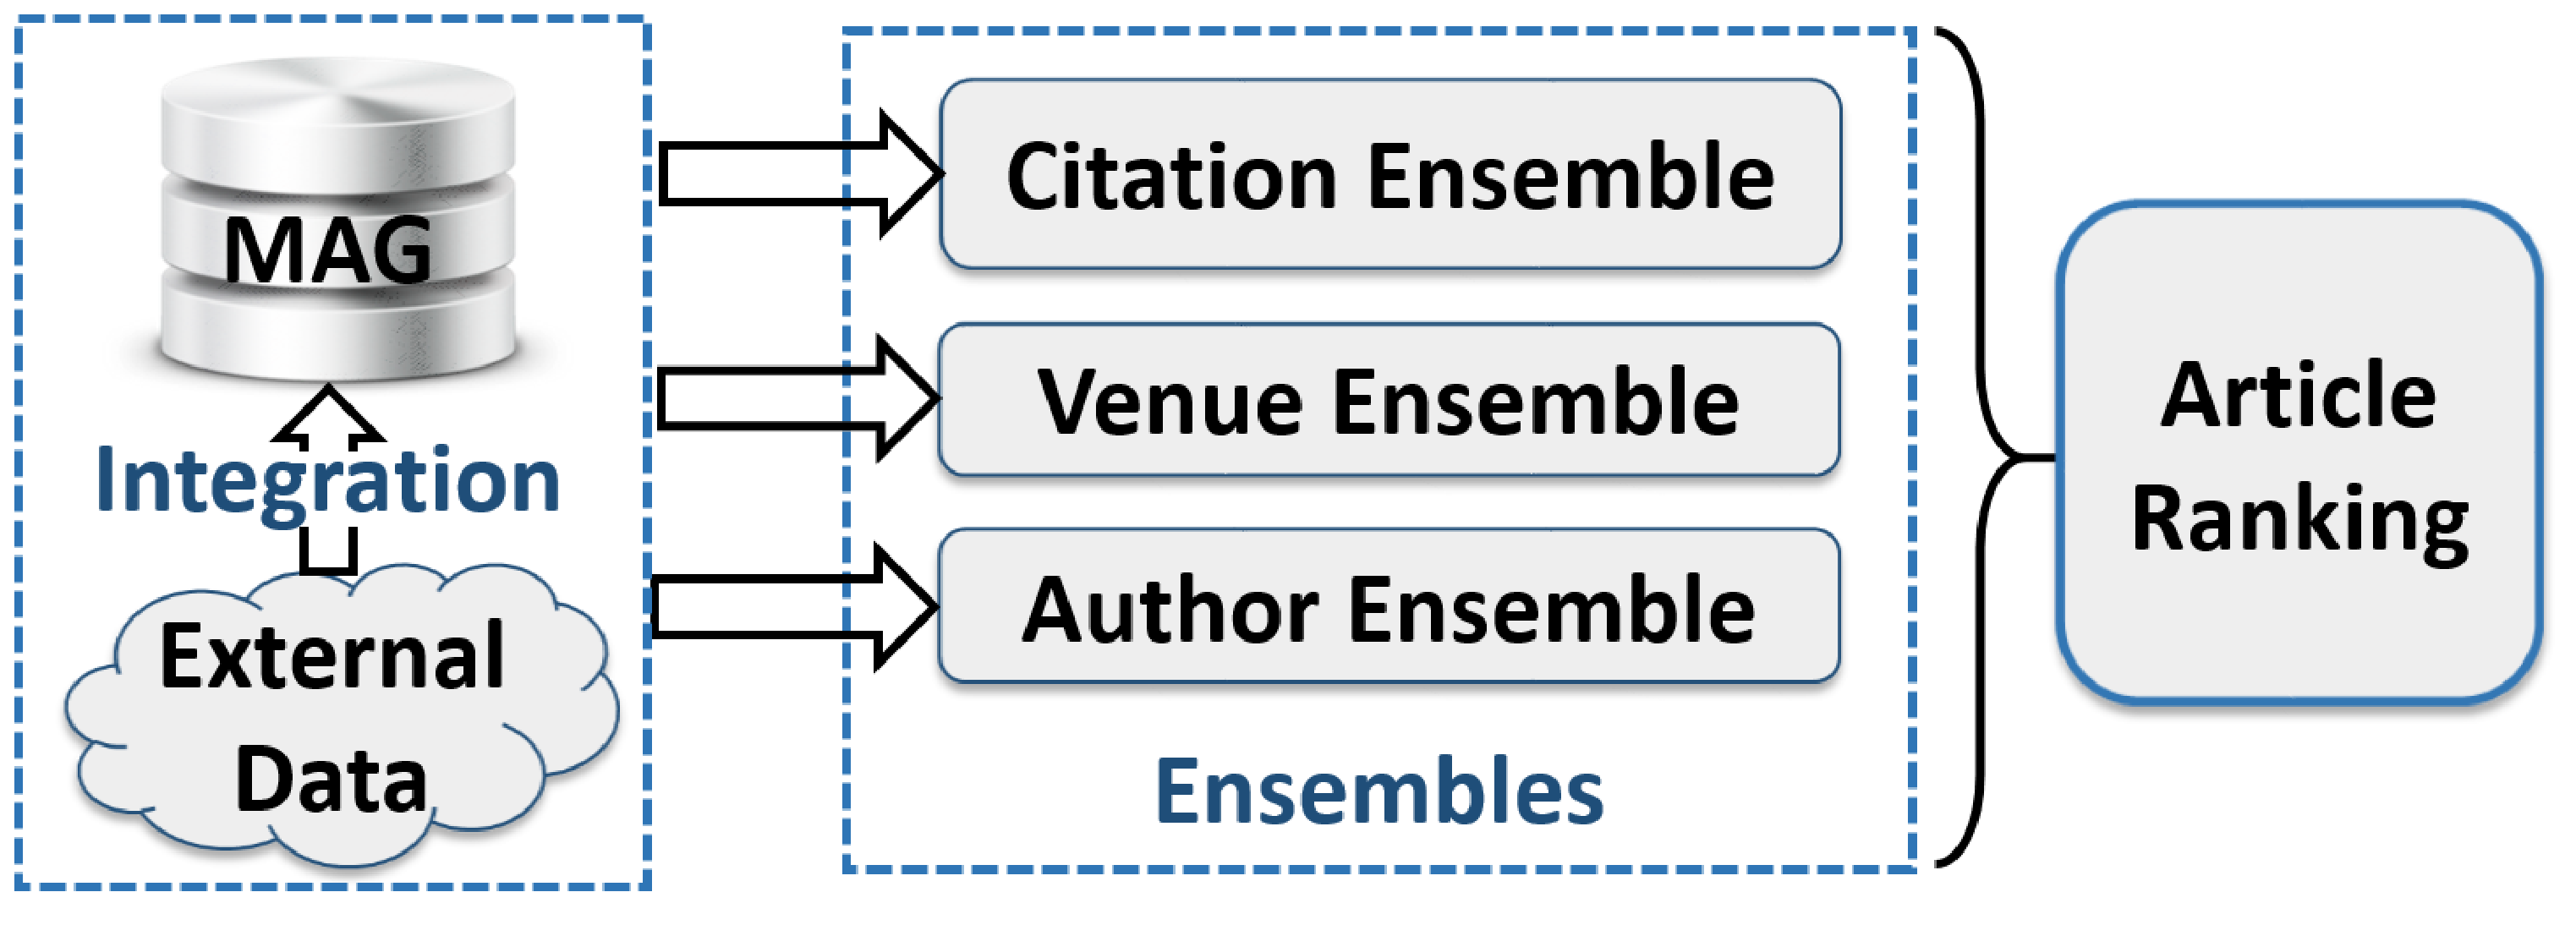
\includegraphics[scale=0.15]{fig/framework.eps}
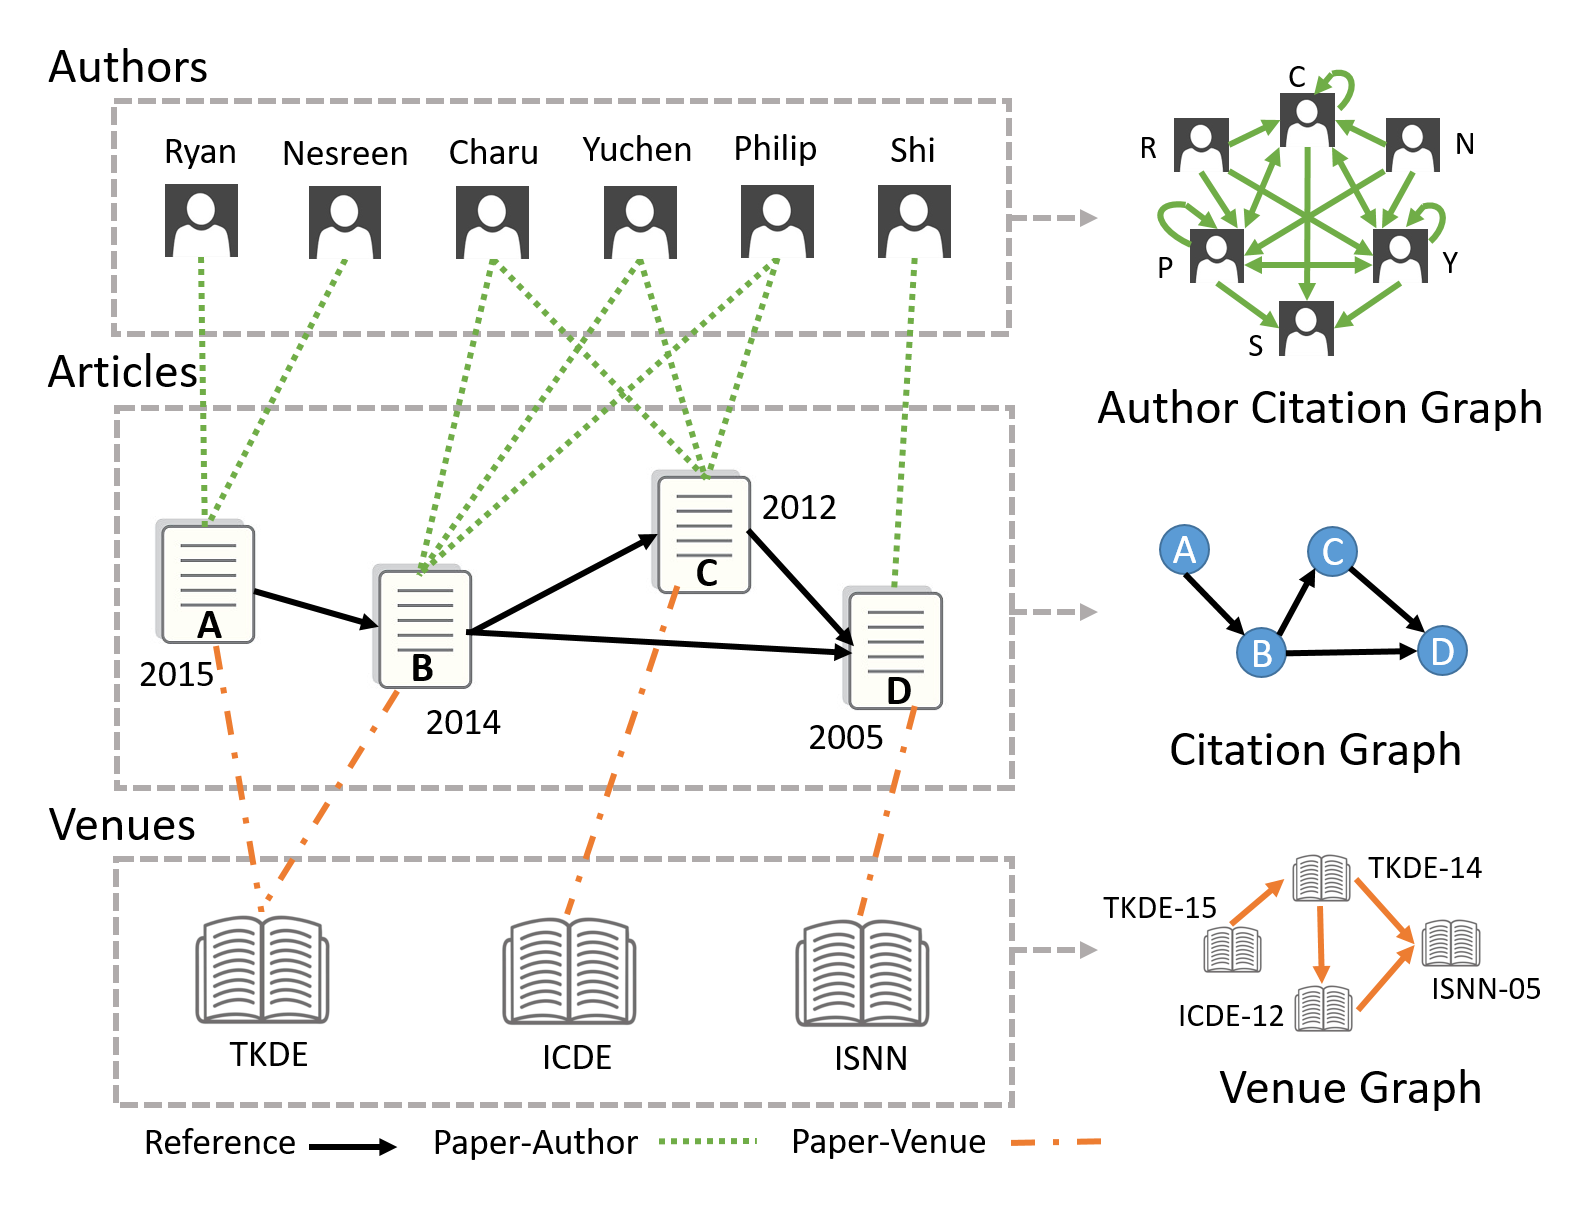
\includegraphics[scale=0.35]{fig/example-graph.eps}
\vspace{-1ex}
\caption{\small An example of graph generation} \label{fig-example-graph}
\vspace{-3ex}
\end{figure}

\begin{figure}[tb!]
\centering
%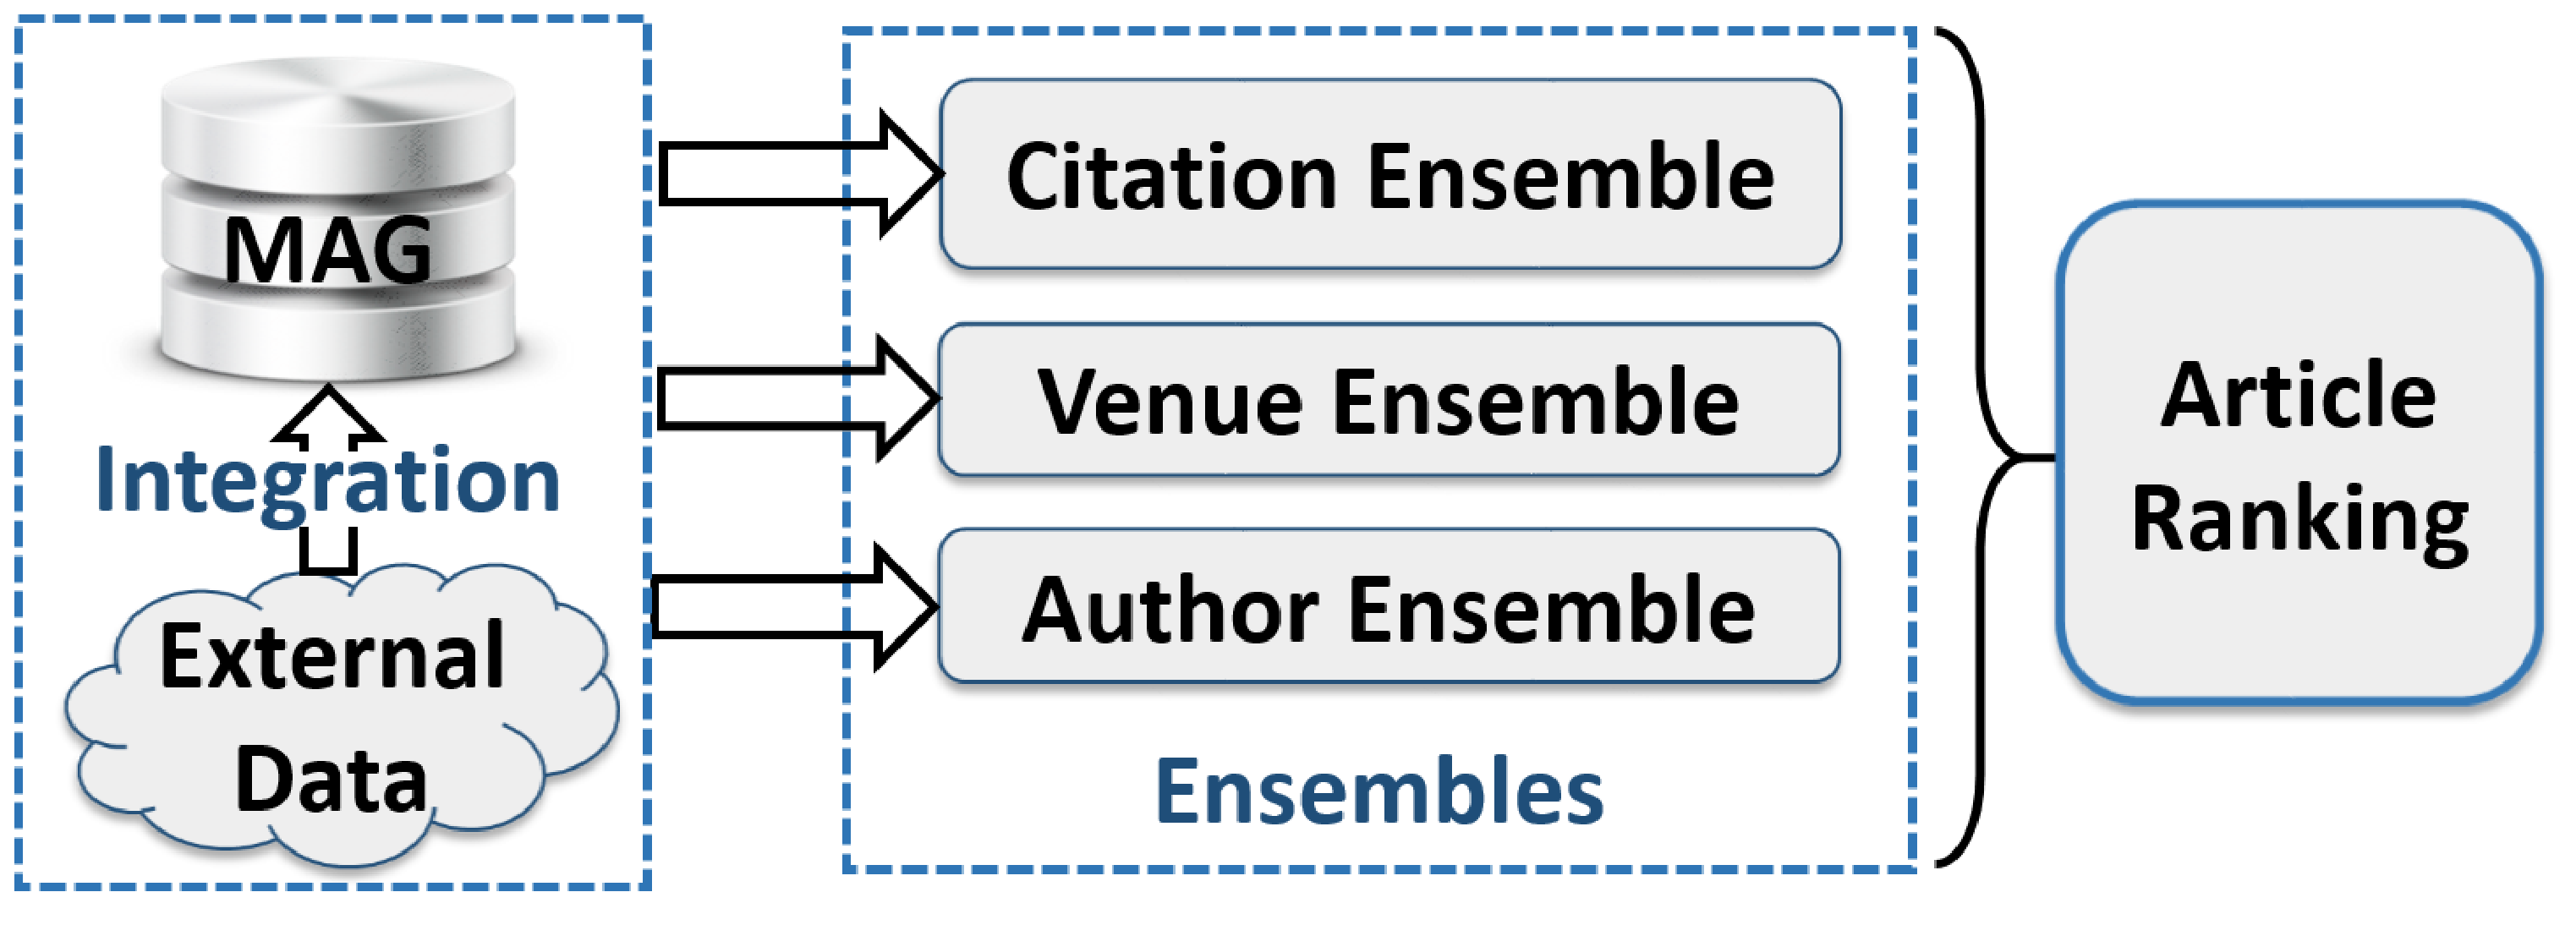
\includegraphics[scale=0.15]{fig/framework.eps}
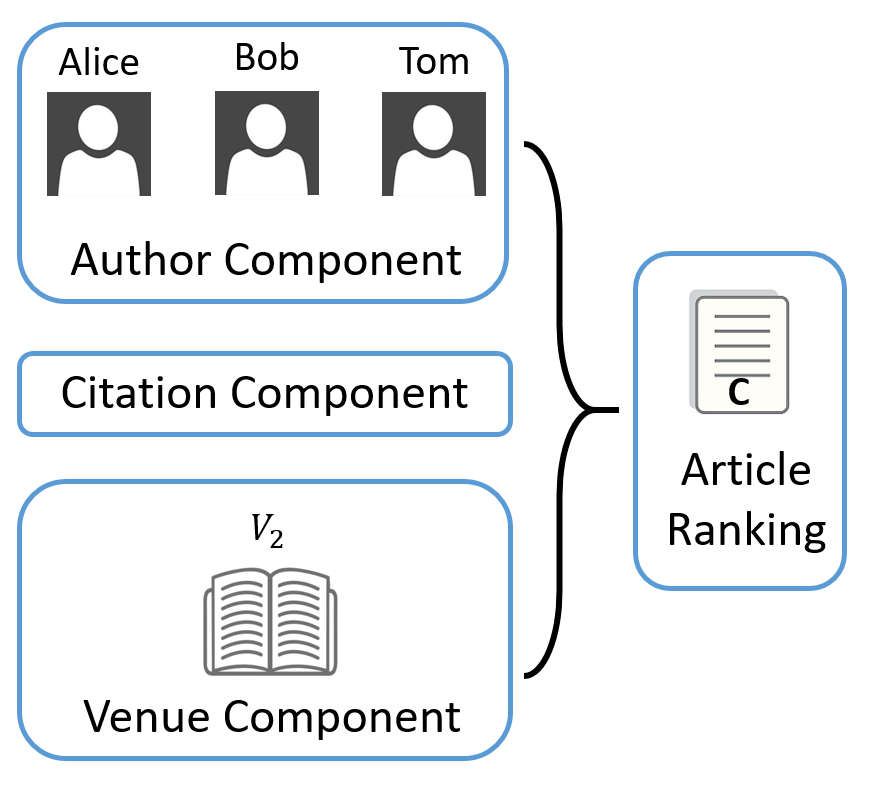
\includegraphics[scale=0.35]{fig/example-ranking.eps}
\vspace{-1ex}
\caption{\small An example of ranking model \ensemblerank} \label{fig-example-model}
\vspace{-3ex}
\end{figure}

%In our model, the importance of scholarly articles is defined as a combination of the prestige and popularity of its associated articles, venues and authors. Intuitively, prestige favors those with many citations soon after the publication of articles for citation component or associated articles for venue and author components, and popularity favors those with recent citations. Both prestige and popularity capture the temporal nature of entities in scholarly data.
In our model, the importance is defined as a combination of the prestige and popularity. Intuitively, prestige favors those with many citations soon after the publication of articles or associated articles of venues and authors, and popularity favors those with recent citations. Both prestige and popularity capture the temporal nature of entities. %in scholarly data.

Our ranking model \ensemblerank,  illustrated in Fig.~\ref{fig-rankmodel}, assembles the importance of article, venue and author entities for scholarly article ranking, which is computed by the citation, venue and author components, respectively.
%
We next introduce the details of the three components.


\begin{example} \label{eg-layer-dag}
Figure~\ref{fig-example-graph} illustrates an example of graph generation. We choose four articles of real-life data to show how to generate the citation graph, venue graph and author citation graph while the original academic graph data only has citation information, author-article relationships, article-venue relationships and time information of articles. As shown in Figure~\ref{fig-example-graph}, the articles A, B, C and D represent "Role Discovery in Networks", "On the Use of Side Information for Mining Text Data", "On Text Clustering with Side Information" and "Efficient streaming text clustering", respectively. We next introduce the details of graph generation.

The citation graph is constructed using the citation information such that each node denotes an individual article and the edge $(A,B)$ denotes that article A have cited article B. The venue graph is constructed using the citation information among venues. As shown in Figure~\ref{fig-example-graph}, each node denotes a venue in a specific year such that TKDE-14 and TKDE-15 are two different nodes. Further, each edge denotes that there are citations between the articles published in the two venues. The author citation graph is constructed using the citation information among authors. As shown in Figure~\ref{fig-example-graph}, the article citation between article A and article B will generate 6 different edges in author citation graph, which makes it much more complicated than citation graph. As a result, the citation graph of 4 articles and 4 edges have generated a author citation graph of 6 nodes and 18 edges (the bidirectional arrow denotes two edges) although the article B and article C have shared same authors.

\end{example}

\begin{example} \label{eg-layer-dag}
Figure~\ref{fig-example-model} illustrates an example of article ranking model. Consider an article $v$ published by authors $t$ and $u$ in venue $k$. 

\end{example}


